% Name: Sequence diagram
% Description: A browser, a server, and a database exchanging messages, with activation bars and replies.
% Tags: sequence diagram, UML, messages, HTTP

\usetikzlibrary{arrows.meta}

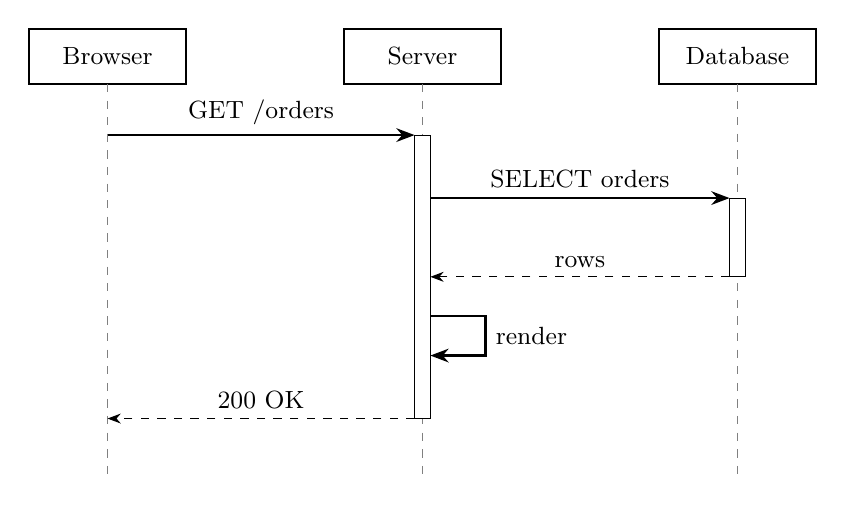
\begin{tikzpicture}[
  every node/.style={font=\small},
  actor/.style={draw, thick, minimum width=20mm, minimum height=7mm},
  active/.style={draw, fill=white},
  call/.style={-{Stealth}, thick},
  reply/.style={-{Stealth}, dashed},
]
  \foreach \x/\name in {0/Browser, 4/Server, 8/Database} {
    \node[actor] at (\x,0) {\name};
    \draw[gray, dashed] (\x,-0.35) -- (\x,-5.4);
  }
  \draw[active] (3.9,-1) rectangle (4.1,-4.6);
  \draw[active] (7.9,-1.8) rectangle (8.1,-2.8);

  \draw[call] (0,-1) -- node[above] {GET /orders} (3.9,-1);
  \draw[call] (4.1,-1.8) -- node[above] {SELECT orders} (7.9,-1.8);
  \draw[reply] (7.9,-2.8) -- node[above] {rows} (4.1,-2.8);
  \draw[call] (4.1,-3.3) -- ++(0.7,0) -- ++(0,-0.5) node[midway, right] {render} -- (4.1,-3.8);
  \draw[reply] (3.9,-4.6) -- node[above] {200 OK} (0,-4.6);
\end{tikzpicture}
